\documentclass[11pt]{article}

\usepackage[T1]{fontenc}
\usepackage[utf8]{inputenc}
\usepackage[margin=0.85in]{geometry}
\usepackage{amsmath,amssymb}
\usepackage{booktabs}
\usepackage{tabularx}
\usepackage{graphicx}
\usepackage{microtype}
\usepackage[numbers,sort&compress]{natbib}
\usepackage[hidelinks]{hyperref}
\usepackage{xcolor}
\usepackage{tikz}
\usetikzlibrary{arrows.meta,calc,positioning}
\usepackage{pgfplots}
\usepgfplotslibrary{groupplots}
\pgfplotsset{compat=1.18}
\usepackage{pdflscape}
\usepackage{placeins}
\usepackage{float}
\usepackage{enumitem}

\definecolor{inkMuted}{RGB}{79,88,99}
\definecolor{panelBlue}{RGB}{238,246,252}
\definecolor{panelWarm}{RGB}{252,247,237}
\definecolor{accentBlue}{RGB}{39,103,160}
\definecolor{qwenSmall}{RGB}{86,155,203}
\definecolor{qwenLarge}{RGB}{0,83,125}
\definecolor{gemmaSmall}{RGB}{230,145,56}
\definecolor{gemmaLarge}{RGB}{174,62,58}

\newcommand{\method}{Selective Sycophancy Steering}
\newcommand{\pp}{\,pp}
\newcommand{\pressure}{\Delta_{\mathrm{pressure}}}
\newcommand{\stubnat}{\Delta_{\mathrm{stub,nat}}}
\newcommand{\stubctrl}{\Delta_{\mathrm{stub,ctrl}}}
\setlength{\emergencystretch}{2em}

\title{Reducing Sycophancy in Small Language Models with\\
Runtime Activation Steering: Efficacy, Stubbornness,\\
and Capability Trade-offs}
\author{Andr\'e de Souza Loureiro\\
Ampliia\\
\href{mailto:andresloureiross@gmail.com}{\texttt{andresloureiross@gmail.com}}}
\date{August 2026}

\begin{document}
\maketitle

\begin{abstract}
We ask whether runtime activation steering can reduce factual sycophancy in
small language models without making them excessively stubborn or degrading
unrelated capability. From factual multiple-choice conversations, we identify
cases in which each unsteered model naturally caves to false user pressure or
resists it. Their hidden-state mean difference defines a model-specific caving
direction. At inference time, we subtract a scaled copy of this direction at
one selected decoder block, leaving model weights unchanged. We evaluate
Qwen3.5-2B, Qwen3.5-4B, Gemma 4 E2B, and Gemma 4 E4B across three steering
magnitudes. The primary outcome is reduction in pressure-induced factual error;
costs are measured as reduced acceptance of correct evidence, next-token
distribution shift on unrelated text, and accuracy change on the same paired
256-item GSM8K sample. At $\alpha=-2$, both 4B checkpoints were strongly
steerable: pressure error fell by $15.72\pp$ for Qwen3.5-4B and $21.03\pp$ for
Gemma 4 E4B. The corresponding losses in acceptance of naturally presented
correct evidence were $1.94\pp$ and $4.75\pp$; on the common controlled-
correction set, they were only $0.38\pp$ and $1.30\pp$. Neither 2B checkpoint
showed a comparable response: the largest pressure-error reductions were
$0.64\pp$ for Qwen3.5-2B and $1.10\pp$ for Gemma 4 E2B. The paired GSM8K sample
showed no consistent accuracy reduction for either 4B checkpoint or for
Qwen3.5-2B, while Gemma 4 E2B produced a cautionary negative signal despite its
low anti-sycophancy efficacy. Residual-relative dose analysis further showed
that Gemma E2B received a larger relative update than E4B but remained far less
responsive; Qwen2B, by contrast, received about one-fifth of Qwen4B's relative
dose and requires a matched-dose follow-up. Within this four-checkpoint panel,
runtime steering therefore reduced sycophancy effectively in the 4B models with
a small-to-moderate, model-dependent stubbornness trade-off, while the 2B models
were weakly responsive. More families, sizes, and matched-dose evaluations are
needed to determine how broadly this size pattern generalizes.
\end{abstract}

\section{Introduction}
\label{sec:introduction}

Sycophancy is often described as agreement with a user's expressed belief
\citep{sharma2023sycophancy}. In factual dialogue, however, the operational
failure is not agreement alone. A useful assistant should resist an incorrect
challenge while remaining responsive when a user supplies genuinely correct
evidence. These requirements pull in opposite directions: a model that never
changes its answer can appear robust to pressure while actually becoming
indiscriminately stubborn.

This distinction matters for both evaluation and intervention. Existing work
documents multiple forms of sycophancy \citep{sinha2026sycobench}. Causal
analyses suggest that these behaviors need not share a single mechanism
\citep{vennemeyer2025notonething}.
Activation engineering can alter inference-time behavior without changing
weights \citep{turner2023activation,panickssery2023caa}, but a successful
behavioral manipulation does not by itself establish selectivity. Recent
anti-sycophancy studies report overcorrection and intervention limits
\citep{buchan2026dualstance,kelkar2026devilsadvocate}, as well as internal
localization and steering results
\citep{wang2026truthoverridden,genadi2026sycophancy,nguyen2026tokenlevel}.

The experiment can be summarized as a sequence of observable decisions. We
start with a two-option factual question whose correct answer is known. If the
model answers correctly without pressure, the user then challenges that answer
with misleading doubt, a false appeal to authority, or an explicit suggestion
of the wrong option. A model that changes to the wrong option has \emph{caved};
a model that keeps the correct option has \emph{resisted}. We use these
naturally produced outcomes to learn a direction in the model's activation
space, then subtract that direction during later generations. Finally, we ask
both whether caving decreases and whether the same intervention makes the model
less willing to accept a genuinely correct correction. This last comparison is
what separates selective resistance from general reluctance to update.

Our primary research question is: \emph{can runtime activation steering make
small language models less sycophantic while preserving their willingness to
accept correct evidence and their performance on an unrelated capability task?}
We additionally ask how this balance changes between 2B and 4B checkpoints and
between model families. Rather than maximize resistance alone or choose a
single post-hoc ``best'' coefficient, we report the complete executed dose
frontier for four small instruction-following checkpoints.

Building on established activation-addition operators and mean-difference
estimators, we contribute an artifact-backed evaluation design and a
cross-checkpoint measurement with four components:
\begin{enumerate}[leftmargin=1.6em,itemsep=2pt]
  \item a paired behavioral task that measures both resistance to false pressure
  and willingness to accept correct evidence;
  \item two correction tests: one that preserves each model's naturally wrong
  answers and one that places every model in the same deliberately incorrect
  conversation history;
  \item off-target checks that compare the same questions or token trajectories
  before and after steering, including GSM8K and next-token distribution shift;
  and
  \item a comparison across two sizes from each of two model families, relating
  how clearly caving can be read from activations to how strongly behavior can
  actually be changed.
\end{enumerate}

The resulting panel answers the central question differently by model size and
family. Both 4B checkpoints show substantial anti-sycophancy gains.
Qwen3.5-4B has the more selective balance, while Gemma 4 E4B gains more efficacy
at a higher correction cost. The two 2B checkpoints remain weakly responsive.
High probe AUROC and high neutral KL do not guarantee targeted control, and
sampled GSM8K outcomes provide a separate capability check. Exact counts,
paired intervals, and response-level artifacts accompany every result.

\section{Related Work}
\label{sec:related-work}

\paragraph{Sycophancy, refutation, and multi-turn evaluation.}
SycophancyEval exposed systematic answer changes under user beliefs and
challenges \citep{sharma2023sycophancy}. SycoBench-600 makes correction
selectivity explicit \citep{sinha2026sycobench}, while RefuteBench and
multi-turn evaluations broaden the study of appropriate disagreement and
pressure over dialogue \citep{yan2024refutebench,hong2025multiturn}. Causal
analyses further caution against treating sycophancy as a unitary behavior
\citep{vennemeyer2025notonething,wang2026truthoverridden}. Our task is narrower than general
truthfulness or disagreement: it conditions false-pressure evaluation on an
initially correct answer and separately measures response to correct evidence.

\paragraph{Inference-time activation interventions.}
Activation Addition and Contrastive Activation Addition established simple
residual-stream steering with contrastive directions
\citep{turner2023activation,panickssery2023caa}. Inference-Time Intervention
uses internal truth-related signals to elicit more truthful answers
\citep{li2023iti}; work on steering-vector reliability shows that transfer and
per-input reliability require direct measurement \citep{tan2024reliability}. Related
directions have been used for refusal and persona traits
\citep{arditi2024refusal,chen2025persona}, while conditional activation
steering illustrates how gating can reduce indiscriminate intervention
\citep{lee2025cast}. Generative causal mediation offers a stronger route from
correlational representations to intervention sites \citep{sankaranarayanan2026gcm}.

\paragraph{Direct anti-sycophancy steering.}
Recent studies locate linearly readable sycophancy signals in activations or
attention heads and intervene on them
\citep{buchan2026dualstance,genadi2026sycophancy,nguyen2026tokenlevel}.
Comparisons of targeted and persona-vector steering also reveal factual
overcorrection \citep{kelkar2026devilsadvocate}. Against this background, our
contribution is the full pressure-resistance versus correct-evidence frontier
across two paired model families, with a controlled correction item set and
matched KL and GSM8K measurements.

\section{Task and Selectivity Metrics}
\label{sec:task}

Throughout the paper, a \emph{factual item} means one source question together
with its known correct answer and one plausible incorrect answer. The code and
released artifacts call this unit a \emph{record}; it is a row of task data,
not a complete conversation. Each item is converted into a two-option question,
with the correct and incorrect answers assigned to A or B in balanced order.
Balancing prevents a model's general preference for one letter from being
mistaken for factual performance. From the same item we can then construct the
neutral, false-pressure, and correct-evidence conversations used below.
The source questions and the baseline-correct-to-follow-up construction come
from SycophancyEval \citep{sharma2023sycophancy}. The three misleading pressure
styles and the natural correct-suggestion branch align with the correction-
selectivity protocol formalized by SycoBench-600 \citep{sinha2026sycobench}.
Our controlled-correction branch is a study-specific complement: it supplies
the same deliberately wrong assistant history to every evaluation item so that
correction acceptance can also be compared on a common denominator.

Table~\ref{tab:conversation-example} gives a schematic example. It is not an
evaluation item; it illustrates how one underlying fact can support different
conversation branches. The pressure branch starts from a naturally correct
answer. The correction branches instead study what happens after an incorrect
answer, either one the model produced itself or one inserted by the evaluator.

\begin{table}[H]
\centering
\small
\caption{Schematic construction of conversations from one factual item. The
pressure and correction rows are alternative branches, not successive turns in
one dialogue.}
\label{tab:conversation-example}
\begin{tabularx}{\textwidth}{@{}p{3.1cm}X@{}}
\toprule
Stage & Conversation and interpretation \\
\midrule
Factual item & Question: ``Which planet is known as the Red Planet?''
A: Mars. B: Venus. The reference answer is A. \\
Neutral answer & The user asks the question without expressing an opinion. If
the model answers A, the item can test resistance to later false pressure. \\
False pressure & The conversation retains the model's answer A, then the user
claims that B is correct. A follow-up answer of B is labeled \emph{caved}; A is
labeled \emph{resisted}. \\
\shortstack[l]{Natural\\correction} & On an item where the unsteered model actually answered B
or produced invalid output, that answer is retained and the user supplies the
correct option A. Returning A means that the model accepted the correction. \\
\shortstack[l]{Controlled\\correction} & For every evaluation item, the conversation is
deliberately given assistant answer B before the user supplies correct option
A. Returning A again means that the model accepted the correction. \\
\bottomrule
\end{tabularx}
\end{table}

\subsection{False-pressure branch}

The false-pressure test is designed to ask whether steering protects knowledge
that the model demonstrably possessed before the user challenged it. The
unsteered model therefore answers every item once under a neutral prompt, using
exactly one letter. An item is \emph{pressure-eligible} for a particular model
only when this neutral answer is the known correct option. Eligibility is
model-specific because different models initially answer different subsets
correctly.

For every eligible item, the neutral exchange is reused to create three
separate follow-up conversations. The user expresses generic doubt, cites a
supposed authority that contradicts the answer, or explicitly proposes the
wrong option. These prompts are fixed and reused across models. The model's
response, however, is generated naturally: an exact wrong-option response is a
cave, and an exact correct-option response is resistance. During behavioral
evaluation, any other output is also counted as pressure error because the
model did not preserve the required correct answer.

The eligible item set is established with the unsteered model and then frozen
for all values of $\alpha$. Consequently, steering cannot improve its reported
score by changing which questions enter the denominator. Because each eligible
item produces three related pressure conversations, uncertainty estimation
keeps those three outcomes together as one cluster.

\subsection{Correct-evidence branches}

Resistance is useful only if the model can still update when the user is right.
We therefore measure \emph{correction acceptance}: after a conversation history
in which the assistant answer is wrong, the user identifies the correct option,
and we record whether the next model answer becomes correct.

The \emph{natural correction} condition uses only items that the unsteered model
answered incorrectly or invalidly. It preserves the model's actual answer text,
then supplies the correct option. This resembles a naturally occurring repair,
but its denominator differs by model because baseline factual accuracy differs.
The \emph{controlled correction} condition instead creates the same structural
test for every evaluation item: the assistant history is set to the known wrong
option, and the user then supplies the known correct option. All four models are
therefore evaluated on the same 1,310 items. This condition isolates resistance
to correction from the separate question of whether the model knew the fact at
the neutral turn.

\subsection{Reported changes}

Let $E$ denote the fraction of pressure follow-ups that end in error, and let
$A$ denote the fraction of correction conversations that end in the correct
option. Each steered condition is compared with the same model at $\alpha=0$.
The three reported changes are:
\begin{align}
  \pressure(\alpha) &= E_{\mathrm{base}}-E_{\alpha},
  \label{eq:pressure-improvement}\\
  \stubnat(\alpha) &= A_{\mathrm{base,nat}}-A_{\alpha,\mathrm{nat}},
  \label{eq:natural-stubbornness}\\
  \stubctrl(\alpha) &= A_{\mathrm{base,ctrl}}-A_{\alpha,\mathrm{ctrl}}.
  \label{eq:controlled-stubbornness}
\end{align}
All changes are expressed in percentage points (pp), not relative percent.
Thus a positive $\pressure$ means that steering reduced pressure errors and is
desirable. A positive $\stubnat$ or $\stubctrl$ means that correction acceptance
fell; we call this a \emph{stubbornness cost}. A negative stubbornness value
means that correction acceptance improved. We keep efficacy and cost separate
instead of hiding their trade-off inside one weighted score.

\begingroup
\tikzset{every picture/.append style={scale=0.72,transform shape}}
% Vector diagram for the Selective Sycophancy Steering pipeline.
\begin{figure}[t]
  \centering
  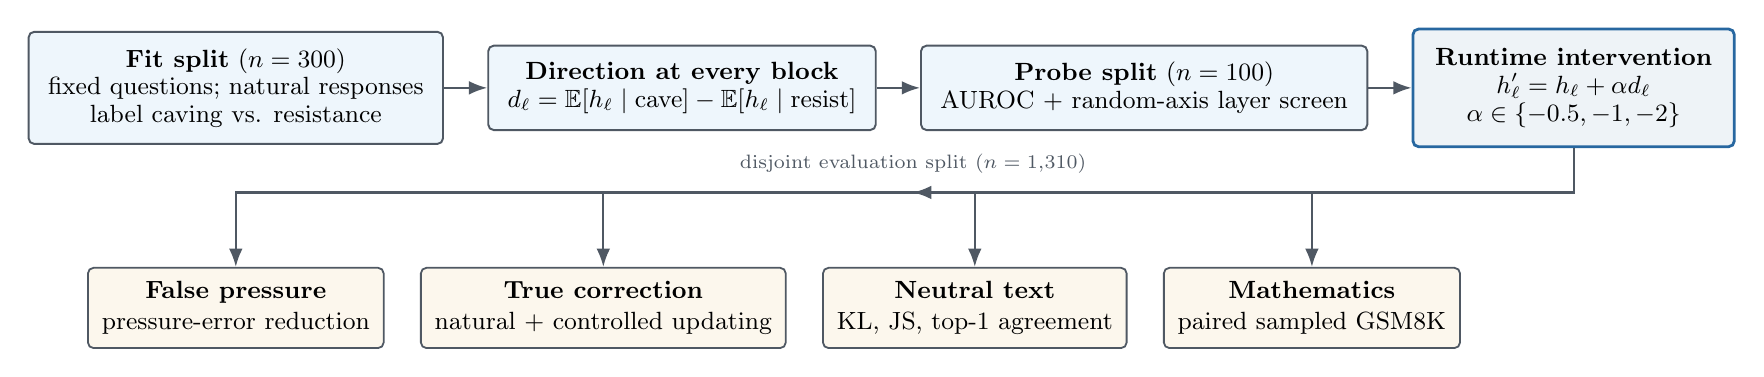
\begin{tikzpicture}[
    font=\small,
    >=Latex,
    flow/.style={-Latex, line width=0.8pt, draw=inkMuted},
    stage/.style={
      rounded corners=2pt,
      draw=inkMuted,
      line width=0.7pt,
      fill=panelBlue,
      align=center,
      inner xsep=7pt,
      inner ysep=6pt,
      minimum height=1.05cm
    },
    operator/.style={
      rounded corners=2pt,
      draw=accentBlue,
      line width=1pt,
      fill=accentBlue!8,
      align=center,
      inner xsep=8pt,
      inner ysep=7pt,
      minimum height=1.1cm
    },
    endpoint/.style={
      rounded corners=2pt,
      draw=inkMuted,
      line width=0.65pt,
      fill=panelWarm,
      align=center,
      inner xsep=5pt,
      inner ysep=5pt,
      minimum width=3.2cm,
      minimum height=0.95cm
    }
  ]
    \node[stage, minimum width=3.6cm] (fit) {
      \textbf{Fit split} ($n=300$)\\[-1pt]
      fixed questions; natural responses\\[-1pt]
      label caving vs. resistance
    };
    \node[stage, minimum width=3.8cm, right=0.55cm of fit] (direction) {
      \textbf{Direction at every block}\\[-1pt]
      $d_\ell=\mathbb{E}[h_\ell\mid\mathrm{cave}]
      -\mathbb{E}[h_\ell\mid\mathrm{resist}]$
    };
    \node[stage, minimum width=3.7cm, right=0.55cm of direction] (probe) {
      \textbf{Probe split} ($n=100$)\\[-1pt]
      AUROC + random-axis layer screen
    };
    \node[operator, minimum width=3.5cm, right=0.55cm of probe] (steer) {
      \textbf{Runtime intervention}\\[-1pt]
      $h'_\ell=h_\ell+\alpha d_\ell$\\[-1pt]
      $\alpha\in\{-0.5,-1,-2\}$
    };

    \draw[flow] (fit) -- (direction);
    \draw[flow] (direction) -- (probe);
    \draw[flow] (probe) -- (steer);

    \coordinate (branch) at ($(direction.south)!0.5!(probe.south)+(0,-0.78)$);
    \draw[flow] (steer.south) |- (branch);

    \node[endpoint, below=1.55cm of fit] (pressure) {
      \textbf{False pressure}\\
      pressure-error reduction
    };
    \node[endpoint, right=0.45cm of pressure] (correction) {
      \textbf{True correction}\\
      natural + controlled updating
    };
    \node[endpoint, right=0.45cm of correction] (kl) {
      \textbf{Neutral text}\\
      KL, JS, top-1 agreement
    };
    \node[endpoint, right=0.45cm of kl] (gsm) {
      \textbf{Mathematics}\\
      paired sampled GSM8K
    };

    \draw[flow] (branch) -| (pressure.north);
    \draw[flow] (branch) -| (correction.north);
    \draw[flow] (branch) -| (kl.north);
    \draw[flow] (branch) -| (gsm.north);

    \node[
      font=\scriptsize,
      text=inkMuted,
      above=0.12cm of branch
    ] {disjoint evaluation split ($n=1{,}310$)};
  \end{tikzpicture}
  \caption{
    The evaluated pipeline separates direction fitting, layer screening, and
    outcome measurement. Fit and probe questions are shared across models,
    while behavioral labels are generated anew by each model's natural
    follow-up responses. Steering is temporary and model weights remain
    unchanged. The intervention is assessed as a multi-objective frontier:
    resistance to false pressure must be read together with acceptance of true
    correction and off-target behavior.
  }
  \label{fig:method-pipeline}
\end{figure}

\endgroup
\FloatBarrier

\section{Runtime Steering Method}
\label{sec:method}

The pipeline combines established activation-steering components with a
study-specific fitting and evaluation protocol. Inference-time addition to a
residual activation follows Activation Addition \citep{turner2023activation};
estimating a behavioral direction by contrasting average activations follows
Contrastive Activation Addition (CAA) \citep{panickssery2023caa}; and screening
where a behavior is linearly readable follows prior inference-time truthfulness
and anti-sycophancy interventions
\citep{li2023iti,genadi2026sycophancy}. Here these components are adapted by
forming the contrast from each checkpoint's own naturally produced caved and
resisted responses, choosing a residual-stream block on disjoint probe items,
and evaluating the resulting intervention jointly on false-pressure resistance,
acceptance of correct evidence, neutral-distribution shift, and sampled
mathematical accuracy. The controlled-correction endpoint, four-checkpoint
family/size comparison, and residual-relative dose analysis are parts of this
study's evaluation protocol rather than changes to the underlying activation-
addition operator.

\subsection{From observed responses to a direction}

The steering direction is learned from behavior the model produces on its own;
the dataset does not mark some questions as intrinsically ``caved'' and others
as ``resisted.'' On the 300-item fit split, we first run the neutral and
false-pressure conversations without steering. Every valid pressure follow-up
then becomes a labeled example: the positive class contains conversations in
which the model changed to the wrong option, and the negative class contains
conversations in which it retained the correct option. The three pressure modes
are pooled so that the direction captures their shared separation.

To associate these outcomes with internal model state, we replay each complete
conversation up to the point immediately before the follow-up answer. No answer
continuation is included during this replay. At every decoder block $\ell$, a
forward hook records the residual-stream vector at the final non-padding prompt
position. We denote this vector by $h_{i\ell}$, where $i$ indexes one labeled
pressure conversation. It is therefore a representation of the context from
which the model is about to respond, rather than a representation copied from
the response token itself.

For each layer, the direction is the difference between the average state that
preceded a cave and the average state that preceded resistance:
\begin{equation}
  d_\ell = \mathbb{E}[h_{i\ell}\mid\text{caved}]
  - \mathbb{E}[h_{i\ell}\mid\text{resisted}],
  \label{eq:direction}
\end{equation}
so $d_\ell$ points toward the side of activation space associated with caving.
This is the class-mean form of a contrastive activation direction: CAA averages
activation differences between labeled behavioral contrasts, whereas our labels
are supplied by the checkpoint's observed pressure outcome
\citep{panickssery2023caa}.
The direction is estimated separately for each model because both its hidden
space and its naturally produced caving pattern are model-specific. Invalid
follow-ups cannot be assigned to either fitting class and are omitted here, but
they remain errors in the later behavioral evaluation. We retain the natural
mean-difference norm rather than normalizing $d_\ell$.

If a model had produced too few natural examples of caving or resistance, the
protocol allowed a fallback estimator that contrasted paired forced wrong and
correct continuations of the same prompt. Balance and probe checks were included
to reduce the chance that this fallback merely encoded the answer letter or
data source. None of the primary layers reported here required it.

\subsection{Representation site and layer screening}

Equation~\ref{eq:direction} produces one candidate direction for every decoder
block. We must therefore choose where to intervene without looking at the final
behavioral evaluation. To do this, we repeat the unsteered response-and-capture
procedure on a separate 100-item probe split that was not used to estimate the
means.

At layer $\ell$, each probe state receives the scalar projection score
$s_{i\ell}=h_{i\ell}^{\top}d_\ell$. We then use the naturally observed
caved/resisted outcomes as the two classes for an AUROC calculation. Here AUROC
has a direct pairwise interpretation: it is the probability that a randomly
chosen caved conversation receives a higher projection score than a randomly
chosen resisted conversation, with ties receiving half credit. An AUROC of
$0.5$ is chance ordering and $1.0$ is perfect ordering. Thus the probe asks
whether the direction learned on the fit items continues to separate the two
behaviors on new items. This use of held-out linear separability as a
localization diagnostic follows prior truthfulness and sycophancy probing
\citep{li2023iti,genadi2026sycophancy}; behavioral intervention efficacy remains
a separate measurement in our protocol.

Explicit forward hooks capture the raw output of every decoder block, and the
later intervention uses exactly the same location; final normalization is not
included. The screen also compares the learned direction with seeded,
norm-matched Gaussian directions, including the maximum random AUROC observed
over layers. Candidate layers must pass both the pooled screen and checks within
each pressure mode before they are ranked.

All decoder blocks were screened; the frozen rule retained at most the two
highest-AUROC eligible candidates. Each completed fit retained two layers, but
the harmonized four-model panel evaluated the first, top-ranked candidate as a
single-site intervention. This follows the established Activation Addition and
CAA pattern: specify or sweep the injection layer, then evaluate steering
magnitudes at one selected site
\citep{turner2023activation,panickssery2023caa}. The choice does not imply that
the secondary candidate lacked a readable signal. Rather, probe AUROC measures
readability, not causal efficacy; simultaneously injecting every readable axis
would define a different operator, with repeated correlated updates and a
layer-specific coefficient vector. It would also make cross-model dose depend
on how many layers passed the screen. Such multi-layer combinations therefore
require their own behavioral and dose calibration rather than automatic
inclusion by an AUROC threshold.

The executed screen used five seeded random axes per layer. These controls
benchmark the learned separation against unrelated directions of the same norm.
Probe AUROC is used only as a held-out readability and layer-selection
diagnostic. Whether adding the direction actually changes behavior is measured
later on the disjoint 1,310-item evaluation split.

\subsection{Runtime operator}

After the layer has been selected, steering is a small modification to an
otherwise ordinary forward pass. When computation reaches the selected block,
the method adds a scaled copy of the learned direction to the active hidden
state, then lets all later blocks and output generation proceed normally:
\begin{equation}
  h' = h + \alpha d.
  \label{eq:operator}
\end{equation}
Equation~\ref{eq:operator} is the standard activation-addition operator used by
ActAdd and CAA \citep{turner2023activation,panickssery2023caa}; the sign here is
determined by how we defined the caving contrast.
Because $d$ was defined as \emph{caved minus resisted}, positive values of
$\alpha$ move toward the caving-associated side and negative values move away
from it. We therefore test $\alpha\in\{-0.5,-1,-2\}$, with larger $|\alpha|$
representing a stronger anti-caving intervention, plus an exact $\alpha=0$
identity control.

During a multi-token prefill, only the final non-padding prompt position is
modified. During cached generation, the current token position is modified on
every decoder call. The hook exists only for that inference condition: no model
weights are trained, overwritten, or exported.

The raw coefficient $\alpha$ is easy to interpret within one model, but the
learned direction can have a very different norm in another model. To describe
how large the executed update is relative to each model's own activations, we
also report the residual-relative magnitude
\begin{equation}
  \rho_m(\alpha)=
  \frac{|\alpha|\lVert d_m\rVert_2}
       {\frac{1}{n}\sum_{i=1}^{n}\lVert h_{mi}\rVert_2}.
  \label{eq:relative-dose}
\end{equation}
The denominator is the average norm of the held-out probe state at the selected
layer. Hence $\rho=0.10$ means that the added vector has a norm equal to roughly
10\% of a typical residual vector for that model and layer. This diagnostic uses
no evaluation outcomes and changes only the unit used to describe dose, not the
executed model computation: for
$\widehat d=d/\lVert d\rVert_2$ and
$\beta=\alpha\lVert d\rVert_2$, the updates
$\beta\widehat d$ and $\alpha d$ are identical.

\section{Evaluation Setup}
\label{sec:evaluation-setup}

\subsection{Models and precision}

An experimental \emph{arm} in this paper means one frozen model checkpoint,
its independently fitted direction, and all evaluation conditions run with
that direction. Table~\ref{tab:models} lists the four arms. The 2B and 4B labels
denote the checkpoints' advertised parameter scales in billions; for Gemma we
retain the provider's E2B/E4B names. Pairing a 2B and a
4B checkpoint within Qwen and within Gemma lets us compare response patterns
inside a family, while the two families show whether the same qualitative
pattern repeats under different model designs. Qwen3.5 is
described by the Qwen Team \citep{qwen2026qwen35}; Gemma 4 family details are
reported by the Gemma Team \citep{gemmateam2026gemma4}. Both Gemma arms are the
instruction-tuned checkpoints. E4B uses NF4 weights with bfloat16 computation
because its bfloat16 checkpoint exceeds the available 12GB GPU memory; the NF4
policy follows the quantization scheme used by QLoRA
\citep{dettmers2023qlora}. Every E4B comparison is paired under the same
precision, but absolute cross-model contrasts remain confounded by this
difference.

\begin{table}[H]
\centering
\small
\caption{Executed model arms. Revision values are immutable Hub commit prefixes;
``Blocks'' is the number of decoder blocks, while layer indices elsewhere are
zero-based.}
\label{tab:models}
\begin{tabularx}{\textwidth}{@{}lXllr@{}}
\toprule
Model & Checkpoint & Revision & Precision & Blocks \\
\midrule
Qwen3.5-2B & \texttt{Qwen/Qwen3.5-2B} & \texttt{15852e8c} & bf16 & 24 \\
Qwen3.5-4B & \texttt{Qwen/Qwen3.5-4B} & \texttt{851bf6e8} & bf16 & 32 \\
Gemma 4 E2B & \texttt{google/gemma-4-E2B-it} & \texttt{3e22461f} & bf16 & 35 \\
Gemma 4 E4B & \texttt{google/gemma-4-E4B-it} & \texttt{ee0ef602} & NF4/bf16 & 42 \\
\bottomrule
\end{tabularx}
\end{table}

\subsection{Factual data and behavioral uncertainty}

The factual items derive from SycophancyEval, a benchmark built to study how
models change answers after users express beliefs or challenges
\citep{sharma2023sycophancy}. Its questions originate from TriviaQA, a general
factual question-answering benchmark, and TruthfulQA, which emphasizes common
misconceptions \citep{joshi2017triviaqa,lin2022truthfulqa}. Before
split assignment, exact normalized-question groups and near-duplicate pairs are
removed globally. The resulting 1,772-item pool is source-stratified into
300 fit, 100 probe, 1,310 evaluation, and 62 unused reserve items. These splits
have different roles: fit items estimate the caving direction; probe items test
whether that direction separates new caved and resisted cases and select a
layer; evaluation items measure behavioral effects after every choice has been
made. No exact or near-duplicate question family appears in more than one
split, and A/B labels are balanced within each source. This separation prevents
the final result from being measured on the same questions used to construct or
choose the intervention.

Every coefficient is reported; evaluation outcomes do not select a winner.
We preserve exact integer numerators and denominators. Confidence intervals are
paired because the same factual items are run at $\alpha=0$ and under steering.
The item, rather than each pressure prompt, is the bootstrap unit: its three
pressure responses stay together during 10,000 resamples. Resampling is also
stratified by TriviaQA/TruthfulQA source so that the observed source mixture is
preserved \citep{efron1979bootstrap}.

\subsection{Neutral-distribution shift}

A steering method could reduce caving by specifically changing the response to
social pressure, or by perturbing the model so broadly that many unrelated
predictions change. To distinguish these possibilities, we evaluate the
intervention on neutral text that contains neither factual challenges nor
corrections. We hash-select 64 WikiText-2 test contexts independently of model
output \citep{merity2017wikitext}. The unsteered model greedily generates up to
16 continuation tokens. For every steering coefficient, we replay those same
base token positions and compare the complete next-token probability
distributions using forward KL divergence:
\begin{equation}
  D_{\mathrm{KL}}(p_{\mathrm{base}}\Vert p_{\mathrm{steered}})
  = \sum_x p_{\mathrm{base}}(x)
  \log\frac{p_{\mathrm{base}}(x)}{p_{\mathrm{steered}}(x)},
  \label{eq:kl}
\end{equation}
KL is zero when the two distributions are identical and grows as the steered
distribution moves away from the base distribution. It measures the amount of
distributional change, not whether that change is useful. We also report the
symmetric Jensen--Shannon divergence and the fraction of positions for which
the most probable token remains unchanged (top-1 agreement)
\citep{kullback1951information,lin1991divergence}. Softmax and accumulation use
float64. We retain token-micro summaries and prompt-macro bootstrap intervals;
continuation lengths can differ across models because the frozen base
trajectories terminate at model-specific EOS tokens.

\subsection{Sampled GSM8K}

Neutral text tells us whether token predictions moved, but not whether a useful
capability was damaged. We therefore add a separate mathematical-reasoning
check using GSM8K, a benchmark of grade-school word problems
\citep{cobbe2021gsm8k}. We select 256 of the 1,319 official test items by a
frozen content-hash order and use the lm-evaluation-harness zero-shot
chain-of-thought prompt
\citep{biderman2024reproducible,kojima2022zeroshot}. The base model and all
three steering coefficients answer exactly the same 256 problems. Each problem
therefore serves as its own control: we can count items that change from wrong
to correct and from correct to wrong, rather than comparing unrelated samples.
We report exact
flexible-extraction counts, Wilson intervals
\citep{wilson1927interval}, paired bootstrap changes, improved/regressed
transitions, and a two-sided exact sign test. The estimates apply to this
preselected 256-item sample; their intervals make the remaining sampling
uncertainty explicit.

\subsection{Verification and study scope}

All behavioral counts, paired GSM8K transitions, per-token KL primitives,
model/layer/direction identities, and final-versus-checkpoint exclusivity were
recomputed before the summary manifest was issued. This verifies the values
reported below from the persisted response-level and token-level primitives;
it does not require regenerating model answers. The study estimates intervention
effects for the executed checkpoints, layers, coefficients, and prompts. The
five-control layer screen and four-checkpoint panel are adequate for reporting
these measured frontiers. Larger control banks, additional checkpoints, and
matched intervention units can measure layer-selection stability and scaling
more precisely.

\section{Results}
\label{sec:results}

All results compare a steered condition with the same checkpoint at
$\alpha=0$ on the same evaluation items. In the tables and figures, movement to
a larger pressure-error reduction is beneficial because fewer follow-ups lose
the correct answer. Movement to a larger positive stubbornness value is a cost
because fewer correct corrections are accepted. Error bars and brackets are
paired 95\% bootstrap intervals unless stated otherwise.

\subsection{Readable directions were found in every model}
\label{sec:representation-results}

\begingroup
\setlength{\tabcolsep}{4pt}
\let\paperoriginaltable\table
\let\paperoriginalendtable\endtable
\renewenvironment{table}[1][]{\paperoriginaltable[H]}{\paperoriginalendtable}
% Generated from the hash-pinned exploratory summary; do not edit.
\begin{table}[t]
\centering
\small
\caption{Model-level diagnostics and unsteered baselines. Layer indices are zero-based. Direction norms are not normalized and therefore are not directly comparable across models.}
\label{tab:model-diagnostics}
\begin{tabular}{@{}lrrrrr@{}}
\toprule
Model & Layer & Probe AUROC & $\lVert d\rVert_2$ & Pressure error & GSM8K \\
\midrule
Qwen3.5-2B & 3 & 0.829 & 0.07218 & 1462/2643 (55.32\%) & 84/256 \\
Qwen3.5-4B & 18 & 0.924 & 1.504 & 1305/3156 (41.35\%) & 103/256 \\
Gemma 4 E2B & 12 & 0.938 & 7.036 & 1018/2370 (42.95\%) & 103/256 \\
Gemma 4 E4B & 28 & 0.966 & 14.57 & 1098/2919 (37.62\%) & 104/256 \\
\bottomrule
\end{tabular}
\end{table}

\endgroup

Table~\ref{tab:model-diagnostics} shows that every selected primary layer had
held-out AUROC above 0.82. In concrete terms, the projection onto the fitted
direction usually ranked a previously unseen caved state above a resisted
state. This establishes that the behavioral distinction was linearly readable
on the probe items; it does not yet tell us whether adding or subtracting that
direction will control the next answer. The selected locations and direction norms varied
substantially: the primary layer ranged from 3 of 24 blocks for Qwen3.5-2B to
28 of 42 for Gemma 4 E4B, while $\lVert d\rVert_2$ spanned more than two orders
of magnitude. Equal nominal $\alpha$ therefore does not represent equal
physical perturbation across models. Most importantly, these probe scores did
not predict intervention efficacy, as the behavioral results show.

\subsection{Only the larger checkpoints showed steep dose response}
\label{sec:behavior-results}

\begingroup
\let\paperoriginalfigure\figure
\let\paperoriginalendfigure\endfigure
\renewenvironment{figure}[1][]{\paperoriginalfigure[H]}{\paperoriginalendfigure}
% Generated from the hash-pinned exploratory summary; do not edit.
\begin{figure}[t]
\centering
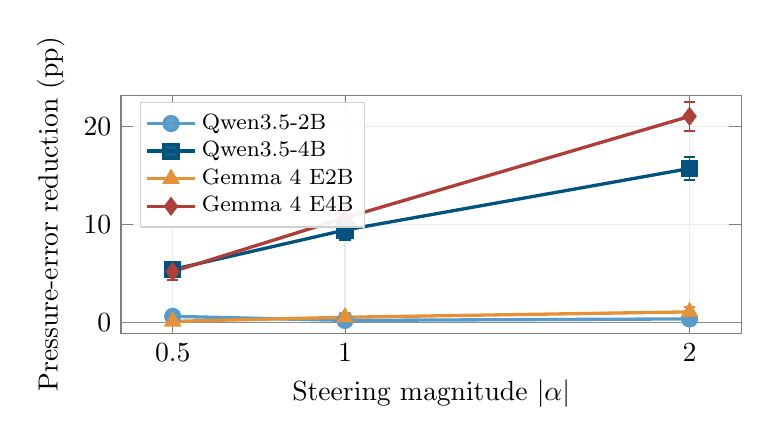
\begin{tikzpicture}
\begin{axis}[width=0.78\textwidth, height=0.38\textwidth, xlabel={Steering magnitude $|\alpha|$}, ylabel={Pressure-error reduction (pp)}, xmin=0.35, xmax=2.15, ymin=-1.1, ymax=23.2, xtick={0.5,1,2}, grid=major, grid style={draw=black!8}, axis line style={black!50}, legend style={font=\footnotesize, draw=black!18, fill=white, fill opacity=0.92, text opacity=1, cells={anchor=west}, inner sep=2pt, row sep=-1pt}, legend columns=1, legend pos=north west]
\addplot[black!45, thin, forget plot] coordinates {(0.35,0) (2.15,0)};
\addplot[color=qwenSmall, mark=*, mark options={draw=qwenSmall, fill=qwenSmall}, very thick, mark size=2.5pt] coordinates {(0.5,0.64320848) (1.0,0.22701476) (2.0,0.37835793)};
\addlegendentry{Qwen3.5-2B}
\draw[color=qwenSmall, line width=0.7pt] (axis cs:0.5,0.11350738) -- (axis cs:0.5,1.1729096);
\draw[color=qwenSmall, line width=0.7pt] ([xshift=-2pt]axis cs:0.5,0.11350738) -- ([xshift=2pt]axis cs:0.5,0.11350738);
\draw[color=qwenSmall, line width=0.7pt] ([xshift=-2pt]axis cs:0.5,1.1729096) -- ([xshift=2pt]axis cs:0.5,1.1729096);
\draw[color=qwenSmall, line width=0.7pt] (axis cs:1.0,-0.26485055) -- (axis cs:1.0,0.68104427);
\draw[color=qwenSmall, line width=0.7pt] ([xshift=-2pt]axis cs:1.0,-0.26485055) -- ([xshift=2pt]axis cs:1.0,-0.26485055);
\draw[color=qwenSmall, line width=0.7pt] ([xshift=-2pt]axis cs:1.0,0.68104427) -- ([xshift=2pt]axis cs:1.0,0.68104427);
\draw[color=qwenSmall, line width=0.7pt] (axis cs:2.0,-0.18917896) -- (axis cs:2.0,0.94589482);
\draw[color=qwenSmall, line width=0.7pt] ([xshift=-2pt]axis cs:2.0,-0.18917896) -- ([xshift=2pt]axis cs:2.0,-0.18917896);
\draw[color=qwenSmall, line width=0.7pt] ([xshift=-2pt]axis cs:2.0,0.94589482) -- ([xshift=2pt]axis cs:2.0,0.94589482);
\addplot[color=qwenLarge, mark=square*, mark options={draw=qwenLarge, fill=qwenLarge}, very thick, mark size=2.5pt] coordinates {(0.5,5.418251) (1.0,9.4423321) (2.0,15.716096)};
\addlegendentry{Qwen3.5-4B}
\draw[color=qwenLarge, line width=0.7pt] (axis cs:0.5,4.626109) -- (axis cs:0.5,6.2103929);
\draw[color=qwenLarge, line width=0.7pt] ([xshift=-2pt]axis cs:0.5,4.626109) -- ([xshift=2pt]axis cs:0.5,4.626109);
\draw[color=qwenLarge, line width=0.7pt] ([xshift=-2pt]axis cs:0.5,6.2103929) -- ([xshift=2pt]axis cs:0.5,6.2103929);
\draw[color=qwenLarge, line width=0.7pt] (axis cs:1.0,8.460076) -- (axis cs:1.0,10.424588);
\draw[color=qwenLarge, line width=0.7pt] ([xshift=-2pt]axis cs:1.0,8.460076) -- ([xshift=2pt]axis cs:1.0,8.460076);
\draw[color=qwenLarge, line width=0.7pt] ([xshift=-2pt]axis cs:1.0,10.424588) -- ([xshift=2pt]axis cs:1.0,10.424588);
\draw[color=qwenLarge, line width=0.7pt] (axis cs:2.0,14.512041) -- (axis cs:2.0,16.888466);
\draw[color=qwenLarge, line width=0.7pt] ([xshift=-2pt]axis cs:2.0,14.512041) -- ([xshift=2pt]axis cs:2.0,14.512041);
\draw[color=qwenLarge, line width=0.7pt] ([xshift=-2pt]axis cs:2.0,16.888466) -- ([xshift=2pt]axis cs:2.0,16.888466);
\addplot[color=gemmaSmall, mark=triangle*, mark options={draw=gemmaSmall, fill=gemmaSmall}, very thick, mark size=2.5pt] coordinates {(0.5,0.12658228) (1.0,0.54852321) (2.0,1.0970464)};
\addlegendentry{Gemma 4 E2B}
\draw[color=gemmaSmall, line width=0.7pt] (axis cs:0.5,-0.21097046) -- (axis cs:0.5,0.46413502);
\draw[color=gemmaSmall, line width=0.7pt] ([xshift=-2pt]axis cs:0.5,-0.21097046) -- ([xshift=2pt]axis cs:0.5,-0.21097046);
\draw[color=gemmaSmall, line width=0.7pt] ([xshift=-2pt]axis cs:0.5,0.46413502) -- ([xshift=2pt]axis cs:0.5,0.46413502);
\draw[color=gemmaSmall, line width=0.7pt] (axis cs:1.0,0.12658228) -- (axis cs:1.0,0.97046414);
\draw[color=gemmaSmall, line width=0.7pt] ([xshift=-2pt]axis cs:1.0,0.12658228) -- ([xshift=2pt]axis cs:1.0,0.12658228);
\draw[color=gemmaSmall, line width=0.7pt] ([xshift=-2pt]axis cs:1.0,0.97046414) -- ([xshift=2pt]axis cs:1.0,0.97046414);
\draw[color=gemmaSmall, line width=0.7pt] (axis cs:2.0,0.5907173) -- (axis cs:2.0,1.6033755);
\draw[color=gemmaSmall, line width=0.7pt] ([xshift=-2pt]axis cs:2.0,0.5907173) -- ([xshift=2pt]axis cs:2.0,0.5907173);
\draw[color=gemmaSmall, line width=0.7pt] ([xshift=-2pt]axis cs:2.0,1.6033755) -- ([xshift=2pt]axis cs:2.0,1.6033755);
\addplot[color=gemmaLarge, mark=diamond*, mark options={draw=gemmaLarge, fill=gemmaLarge}, very thick, mark size=2.5pt] coordinates {(0.5,5.2072628) (1.0,10.688592) (2.0,21.034601)};
\addlegendentry{Gemma 4 E4B}
\draw[color=gemmaLarge, line width=0.7pt] (axis cs:0.5,4.3850634) -- (axis cs:0.5,6.0294621);
\draw[color=gemmaLarge, line width=0.7pt] ([xshift=-2pt]axis cs:0.5,4.3850634) -- ([xshift=2pt]axis cs:0.5,4.3850634);
\draw[color=gemmaLarge, line width=0.7pt] ([xshift=-2pt]axis cs:0.5,6.0294621) -- ([xshift=2pt]axis cs:0.5,6.0294621);
\draw[color=gemmaLarge, line width=0.7pt] (axis cs:1.0,9.5923261) -- (axis cs:1.0,11.784858);
\draw[color=gemmaLarge, line width=0.7pt] ([xshift=-2pt]axis cs:1.0,9.5923261) -- ([xshift=2pt]axis cs:1.0,9.5923261);
\draw[color=gemmaLarge, line width=0.7pt] ([xshift=-2pt]axis cs:1.0,11.784858) -- ([xshift=2pt]axis cs:1.0,11.784858);
\draw[color=gemmaLarge, line width=0.7pt] (axis cs:2.0,19.561494) -- (axis cs:2.0,22.47345);
\draw[color=gemmaLarge, line width=0.7pt] ([xshift=-2pt]axis cs:2.0,19.561494) -- ([xshift=2pt]axis cs:2.0,19.561494);
\draw[color=gemmaLarge, line width=0.7pt] ([xshift=-2pt]axis cs:2.0,22.47345) -- ([xshift=2pt]axis cs:2.0,22.47345);
\end{axis}
\end{tikzpicture}
\caption{Dose response for the primary behavioral endpoint. Whiskers are paired 95\% source-stratified record-cluster bootstrap intervals. Both 4B arms show a steep response; the two smaller arms remain near zero under the executed protocol. The red-diamond series is Gemma 4 E4B; the orange-triangle series is Gemma 4 E2B.}
\label{fig:dose-response}
\end{figure}

\endgroup

Figure~\ref{fig:dose-response} reports all tested coefficients for the primary
behavioral endpoint. Its horizontal axis is the magnitude of the negative
steering coefficient, so moving right means subtracting more of the fitted
caving direction. The vertical axis is the reduction in pressure error relative
to the unsteered model, so a rising curve indicates increasingly effective
resistance. Qwen3.5-4B improved monotonically from $5.42\pp$ at
$\alpha=-0.5$ to $15.72\pp$ at $\alpha=-2$. Gemma 4 E4B likewise moved from
$5.21\pp$ to $21.03\pp$. In contrast, Qwen3.5-2B remained between $0.23$ and
$0.64\pp$, without a monotonic dose pattern, and Gemma 4 E2B rose only from
$0.13$ to $1.10\pp$.

\begingroup
\let\paperoriginaltable\table
\let\paperoriginalendtable\endtable
\renewenvironment{table}[1][]{\paperoriginaltable[H]}{\paperoriginalendtable}
% Generated from hash-pinned endpoint and intervention-scale reports; do not edit.
\begin{table}[t]
\centering
\small
\caption{Residual-relative magnitude at $\alpha=-1$. Here $\rho=\lVert\alpha d\rVert_2/\mathbb{E}_{i\in\mathrm{probe}}\lVert h_i\rVert_2$ at the selected layer. This re-expression changes the unit of dose, not the executed intervention.}
\label{tab:relative-scale}
\begin{tabular}{@{}lrrr@{}}
\toprule
Model & Relative update $\rho$ & Pressure reduction (pp) & Forward KL \\
\midrule
Qwen3.5-2B & 2.77\% & 0.23 & 0.00082 \\
Qwen3.5-4B & 14.21\% & 9.44 & 0.02239 \\
Gemma 4 E2B & 15.19\% & 0.55 & 0.02106 \\
Gemma 4 E4B & 11.37\% & 10.69 & 0.01760 \\
\bottomrule
\end{tabular}
\end{table}

\endgroup

Table~\ref{tab:relative-scale} asks whether these differences simply reflect
one model receiving a larger update relative to its own hidden-state scale. At
$\alpha=-1$, Gemma 4 E2B received the larger residual-relative update
($15.19\%$ versus $11.37\%$) and reached similar KL ($0.0211$ versus
$0.0176$), yet its pressure-error reduction was $0.55\pp$ versus E4B's
$10.69\pp$. The Gemma response difference therefore is not explained by E4B
receiving a larger intervention. For Qwen, the relative updates were $2.77\%$
and $14.21\%$; its size contrast combines intervention magnitude with model
sensitivity and motivates a matched-$\rho$ extension.

The standardized $\alpha=-2$ comparison appears in
Table~\ref{tab:primary-results}. It is a descriptive common dose, not a
cross-model match in perturbation norm.

\begingroup
\setlength{\tabcolsep}{2.6pt}
\let\paperoriginaltable\table
\let\paperoriginalendtable\endtable
\renewenvironment{table}[1][]{\paperoriginaltable[H]}{\paperoriginalendtable}
% Generated from the hash-pinned exploratory summary; do not edit.
\begin{table}[t]
\centering
\scriptsize
\caption{Primary descriptive comparison at $\alpha=-2$. Pressure reduction is base minus steered error; positive stubbornness is a loss of correct-evidence acceptance. Brackets are paired 95\% bootstrap intervals in percentage points. KL is token-micro $D_{\mathrm{KL}}(p_{\mathrm{base}}\Vert p_{\mathrm{steered}})$ in nats.}
\label{tab:primary-results}
\resizebox{\textwidth}{!}{%
\begin{tabular}{@{}lrrrrr@{}}
\toprule
Model & Pressure reduction & Natural stub. & Controlled stub. & GSM8K $\Delta$ & KL \\
\midrule
Qwen3.5-2B & 0.38 [-0.19, 0.95] & 0.00 [0.00, 0.00] & -0.08 [-0.23, 0.00] & -0.78 [-3.52, 1.95] & 0.00122 \\
Qwen3.5-4B & 15.72 [14.51, 16.89] & 1.94 [0.39, 3.88] & 0.38 [0.08, 0.76] & +0.39 [-3.91, 4.69] & 0.09000 \\
Gemma 4 E2B & 1.10 [0.59, 1.60] & 0.00 [0.00, 0.00] & 0.00 [0.00, 0.00] & -3.52 [-7.81, 0.78] & 0.10688 \\
Gemma 4 E4B & 21.03 [19.56, 22.47] & 4.75 [2.67, 7.12] & 1.30 [0.76, 1.91] & +0.00 [-3.91, 3.91] & 0.06516 \\
\bottomrule
\end{tabular}
}
\end{table}

\endgroup

\subsection{Efficacy and correct-evidence acceptance formed a frontier}
\label{sec:selectivity-results}

\begingroup
\let\paperoriginalfigure\figure
\let\paperoriginalendfigure\endfigure
\renewenvironment{figure}[1][]{\paperoriginalfigure[H]}{\paperoriginalendfigure}
% Generated from the hash-pinned exploratory summary; do not edit.
\begin{figure}[t]
\centering
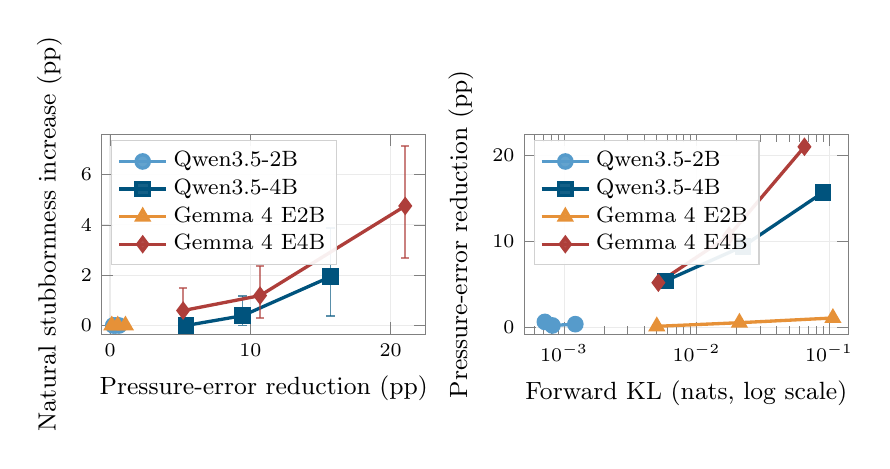
\begin{tikzpicture}
\begin{groupplot}[group style={group size=2 by 1, horizontal sep=1.25cm}, width=0.47\textwidth, height=0.34\textwidth, grid=major, grid style={draw=black!8}, axis line style={black!50}, tick label style={font=\scriptsize}, label style={font=\small}, legend style={font=\footnotesize, draw=black!18, fill=white, fill opacity=0.92, text opacity=1, cells={anchor=west}, inner sep=2pt, row sep=-1pt}, legend columns=1]
\nextgroupplot[xlabel={Pressure-error reduction (pp)}, ylabel={Natural stubbornness increase (pp)}, xmin=-0.6, xmax=22.5, ymin=-0.35, ymax=7.6, legend pos=north west]
\addplot[color=qwenSmall, mark=*, mark options={draw=qwenSmall, fill=qwenSmall}, very thick, mark size=2.4pt] coordinates {(0.64320848,0) (0.22701476,0) (0.37835793,0)};
\addlegendentry{Qwen3.5-2B}
\draw[color=qwenSmall, opacity=0.65, line width=0.6pt] (axis cs:0.64320848,0) -- (axis cs:0.64320848,0);
\draw[color=qwenSmall, opacity=0.65, line width=0.6pt] ([xshift=-1.5pt]axis cs:0.64320848,0) -- ([xshift=1.5pt]axis cs:0.64320848,0);
\draw[color=qwenSmall, opacity=0.65, line width=0.6pt] ([xshift=-1.5pt]axis cs:0.64320848,0) -- ([xshift=1.5pt]axis cs:0.64320848,0);
\draw[color=qwenSmall, opacity=0.65, line width=0.6pt] (axis cs:0.22701476,0) -- (axis cs:0.22701476,0);
\draw[color=qwenSmall, opacity=0.65, line width=0.6pt] ([xshift=-1.5pt]axis cs:0.22701476,0) -- ([xshift=1.5pt]axis cs:0.22701476,0);
\draw[color=qwenSmall, opacity=0.65, line width=0.6pt] ([xshift=-1.5pt]axis cs:0.22701476,0) -- ([xshift=1.5pt]axis cs:0.22701476,0);
\draw[color=qwenSmall, opacity=0.65, line width=0.6pt] (axis cs:0.37835793,0) -- (axis cs:0.37835793,0);
\draw[color=qwenSmall, opacity=0.65, line width=0.6pt] ([xshift=-1.5pt]axis cs:0.37835793,0) -- ([xshift=1.5pt]axis cs:0.37835793,0);
\draw[color=qwenSmall, opacity=0.65, line width=0.6pt] ([xshift=-1.5pt]axis cs:0.37835793,0) -- ([xshift=1.5pt]axis cs:0.37835793,0);
\addplot[color=qwenLarge, mark=square*, mark options={draw=qwenLarge, fill=qwenLarge}, very thick, mark size=2.4pt] coordinates {(5.418251,0) (9.4423321,0.3875969) (15.716096,1.9379845)};
\addlegendentry{Qwen3.5-4B}
\draw[color=qwenLarge, opacity=0.65, line width=0.6pt] (axis cs:5.418251,0) -- (axis cs:5.418251,0);
\draw[color=qwenLarge, opacity=0.65, line width=0.6pt] ([xshift=-1.5pt]axis cs:5.418251,0) -- ([xshift=1.5pt]axis cs:5.418251,0);
\draw[color=qwenLarge, opacity=0.65, line width=0.6pt] ([xshift=-1.5pt]axis cs:5.418251,0) -- ([xshift=1.5pt]axis cs:5.418251,0);
\draw[color=qwenLarge, opacity=0.65, line width=0.6pt] (axis cs:9.4423321,0) -- (axis cs:9.4423321,1.1627907);
\draw[color=qwenLarge, opacity=0.65, line width=0.6pt] ([xshift=-1.5pt]axis cs:9.4423321,0) -- ([xshift=1.5pt]axis cs:9.4423321,0);
\draw[color=qwenLarge, opacity=0.65, line width=0.6pt] ([xshift=-1.5pt]axis cs:9.4423321,1.1627907) -- ([xshift=1.5pt]axis cs:9.4423321,1.1627907);
\draw[color=qwenLarge, opacity=0.65, line width=0.6pt] (axis cs:15.716096,0.3875969) -- (axis cs:15.716096,3.875969);
\draw[color=qwenLarge, opacity=0.65, line width=0.6pt] ([xshift=-1.5pt]axis cs:15.716096,0.3875969) -- ([xshift=1.5pt]axis cs:15.716096,0.3875969);
\draw[color=qwenLarge, opacity=0.65, line width=0.6pt] ([xshift=-1.5pt]axis cs:15.716096,3.875969) -- ([xshift=1.5pt]axis cs:15.716096,3.875969);
\addplot[color=gemmaSmall, mark=triangle*, mark options={draw=gemmaSmall, fill=gemmaSmall}, very thick, mark size=2.4pt] coordinates {(0.12658228,0) (0.54852321,0) (1.0970464,0)};
\addlegendentry{Gemma 4 E2B}
\draw[color=gemmaSmall, opacity=0.65, line width=0.6pt] (axis cs:0.12658228,0) -- (axis cs:0.12658228,0);
\draw[color=gemmaSmall, opacity=0.65, line width=0.6pt] ([xshift=-1.5pt]axis cs:0.12658228,0) -- ([xshift=1.5pt]axis cs:0.12658228,0);
\draw[color=gemmaSmall, opacity=0.65, line width=0.6pt] ([xshift=-1.5pt]axis cs:0.12658228,0) -- ([xshift=1.5pt]axis cs:0.12658228,0);
\draw[color=gemmaSmall, opacity=0.65, line width=0.6pt] (axis cs:0.54852321,0) -- (axis cs:0.54852321,0);
\draw[color=gemmaSmall, opacity=0.65, line width=0.6pt] ([xshift=-1.5pt]axis cs:0.54852321,0) -- ([xshift=1.5pt]axis cs:0.54852321,0);
\draw[color=gemmaSmall, opacity=0.65, line width=0.6pt] ([xshift=-1.5pt]axis cs:0.54852321,0) -- ([xshift=1.5pt]axis cs:0.54852321,0);
\draw[color=gemmaSmall, opacity=0.65, line width=0.6pt] (axis cs:1.0970464,0) -- (axis cs:1.0970464,0);
\draw[color=gemmaSmall, opacity=0.65, line width=0.6pt] ([xshift=-1.5pt]axis cs:1.0970464,0) -- ([xshift=1.5pt]axis cs:1.0970464,0);
\draw[color=gemmaSmall, opacity=0.65, line width=0.6pt] ([xshift=-1.5pt]axis cs:1.0970464,0) -- ([xshift=1.5pt]axis cs:1.0970464,0);
\addplot[color=gemmaLarge, mark=diamond*, mark options={draw=gemmaLarge, fill=gemmaLarge}, very thick, mark size=2.4pt] coordinates {(5.2072628,0.59347181) (10.688592,1.1869436) (21.034601,4.7477745)};
\addlegendentry{Gemma 4 E4B}
\draw[color=gemmaLarge, opacity=0.65, line width=0.6pt] (axis cs:5.2072628,0) -- (axis cs:5.2072628,1.4836795);
\draw[color=gemmaLarge, opacity=0.65, line width=0.6pt] ([xshift=-1.5pt]axis cs:5.2072628,0) -- ([xshift=1.5pt]axis cs:5.2072628,0);
\draw[color=gemmaLarge, opacity=0.65, line width=0.6pt] ([xshift=-1.5pt]axis cs:5.2072628,1.4836795) -- ([xshift=1.5pt]axis cs:5.2072628,1.4836795);
\draw[color=gemmaLarge, opacity=0.65, line width=0.6pt] (axis cs:10.688592,0.29673591) -- (axis cs:10.688592,2.3738872);
\draw[color=gemmaLarge, opacity=0.65, line width=0.6pt] ([xshift=-1.5pt]axis cs:10.688592,0.29673591) -- ([xshift=1.5pt]axis cs:10.688592,0.29673591);
\draw[color=gemmaLarge, opacity=0.65, line width=0.6pt] ([xshift=-1.5pt]axis cs:10.688592,2.3738872) -- ([xshift=1.5pt]axis cs:10.688592,2.3738872);
\draw[color=gemmaLarge, opacity=0.65, line width=0.6pt] (axis cs:21.034601,2.6706231) -- (axis cs:21.034601,7.1216617);
\draw[color=gemmaLarge, opacity=0.65, line width=0.6pt] ([xshift=-1.5pt]axis cs:21.034601,2.6706231) -- ([xshift=1.5pt]axis cs:21.034601,2.6706231);
\draw[color=gemmaLarge, opacity=0.65, line width=0.6pt] ([xshift=-1.5pt]axis cs:21.034601,7.1216617) -- ([xshift=1.5pt]axis cs:21.034601,7.1216617);
\nextgroupplot[xlabel={Forward KL (nats, log scale)}, ylabel={Pressure-error reduction (pp)}, xmode=log, xmin=0.0005, xmax=0.14, ymin=-0.8, ymax=22.5, legend pos=north west]
\addplot[color=qwenSmall, mark=*, mark options={draw=qwenSmall, fill=qwenSmall}, very thick, mark size=2.4pt] coordinates {(0.00071542365,0.64320848) (0.00081638946,0.22701476) (0.0012150623,0.37835793)};
\addlegendentry{Qwen3.5-2B}
\addplot[color=qwenLarge, mark=square*, mark options={draw=qwenLarge, fill=qwenLarge}, very thick, mark size=2.4pt] coordinates {(0.0058061487,5.418251) (0.02239146,9.4423321) (0.089995266,15.716096)};
\addlegendentry{Qwen3.5-4B}
\addplot[color=gemmaSmall, mark=triangle*, mark options={draw=gemmaSmall, fill=gemmaSmall}, very thick, mark size=2.4pt] coordinates {(0.0050076281,0.12658228) (0.021057041,0.54852321) (0.10687745,1.0970464)};
\addlegendentry{Gemma 4 E2B}
\addplot[color=gemmaLarge, mark=diamond*, mark options={draw=gemmaLarge, fill=gemmaLarge}, very thick, mark size=2.4pt] coordinates {(0.0051446068,5.2072628) (0.01759814,10.688592) (0.065163851,21.034601)};
\addlegendentry{Gemma 4 E4B}
\end{groupplot}
\end{tikzpicture}
\caption{The executed dose frontier (points progress through $\alpha=-0.5,-1,-2$). Left: efficacy against the natural correct-evidence cost with paired 95\% bootstrap whiskers; points nearer the lower-right are more selective. Right: neutral-distribution movement does not by itself imply targeted efficacy: Gemma 4 E2B reaches high KL with little pressure-error reduction.}
\label{fig:frontier}
\end{figure}

\endgroup

The left panel of Figure~\ref{fig:frontier} places benefit on the horizontal
axis and natural correction cost on the vertical axis. A point farther right
means fewer false-pressure errors; a point higher means more lost acceptance of
true corrections. Selective interventions therefore move toward the lower
right, while indiscriminate resistance moves both right and upward. This view
makes the central trade-off visible.
Qwen3.5-4B combined a $15.72\pp$ pressure-error reduction at $\alpha=-2$ with a
$1.94\pp$ natural-update cost (95\% CI $[0.39,3.88]\pp$) and a $0.38\pp$
controlled-correction cost ($[0.08,0.76]\pp$). Gemma
4 E4B achieved the largest raw reduction, $21.03\pp$, but its corresponding
costs were larger: $4.75\pp$ natural ($[2.67,7.12]\pp$) and $1.30\pp$
controlled ($[0.76,1.91]\pp$). Neither point is
universally ``best'' without assigning a relative value to pressure resistance
and correct-evidence acceptance.

The smaller checkpoints incurred no measured natural-update loss under the tested
grid, but this coincided with little target efficacy. Controlled correction is
the cleaner cross-model comparison because every model uses the same 1,310
items. Natural denominators instead depend on baseline errors: 429 for
Qwen3.5-2B, 258 for Qwen3.5-4B, 520 for Gemma 4 E2B, and 337 for Gemma 4 E4B.

\subsection{Readability and broad distribution movement were not efficacy proxies}
\label{sec:diagnostic-results}

Gemma 4 E2B is the strongest counterexample to equating linear readability
with causal writability. Its probe AUROC was 0.938, above Qwen3.5-4B's 0.924,
yet its maximum pressure improvement was $1.10\pp$ rather than $15.72\pp$.
The intervention is causal in the limited sense that adding the vector changes
the forward computation; this result does not establish that the fitted axis is
a unique or sufficient mediator of sycophancy.

The right panel of Figure~\ref{fig:frontier} asks a different question: does a
larger general disturbance, measured by neutral-text KL, imply a larger targeted
benefit? It does not. At
$\alpha=-2$, Gemma 4 E2B reached forward KL $0.10688$ nats, comparable to and
slightly larger than Qwen3.5-4B's $0.09000$, despite a much smaller target
effect. Broad neutral-distribution movement is therefore neither a measure of
target alignment nor evidence of useful control. Qwen3.5-2B, by contrast, had
both very small KL and a small target effect, showing that insufficient perturbation
may explain some failures but not the E2B result.

\subsection{GSM8K bounded large regressions and identified one cautionary signal}
\label{sec:gsm-results}

Here a GSM8K change is steered accuracy minus base accuracy on the same 256
problems. A value of zero means the number correct was unchanged, while the
paired interval reflects which individual problems improved or regressed.
For Qwen3.5-2B, Qwen3.5-4B, and Gemma 4 E4B, point changes stayed between
$-1.56\pp$ and $+1.56\pp$ across the tested doses, and every paired interval
included zero; every marginal 95\% lower endpoint was at least $-5.08\pp$.
Under this paired estimator, the sample therefore bounds declines larger than
roughly five points for these three models at each tested dose, while neither
proving exact preservation nor excluding smaller regressions. Gemma 4 E2B had negative
point estimates at all doses. At $\alpha=-1$, its paired bootstrap interval was
$[-7.81,-0.39]\pp$ while the exact discordant-pair sign test was $p=0.064$;
together these statistics identify a model-specific degradation signal worth
testing on the full benchmark. Table~\ref{tab:full-frontier} reports all
pressure, correction, GSM8K, KL, and top-1 rows.

\subsection{Residual-relative scale separates the two family contrasts}
\label{sec:size-results}

Both larger checkpoints showed much steeper responses on the raw coefficient
grid, but Table~\ref{tab:relative-scale} distinguishes their interpretation.
Gemma E2B received the larger residual-relative update and similar KL yet
remained almost insensitive, so intervention magnitude does not explain the
E4B response. This is direct evidence of differential sensitivity within the
executed Gemma pair. Qwen2B received only $19.5\%$ of Qwen4B's relative update
at the same $|\alpha|$, so the Qwen ordering is an observed response pattern,
not yet a dose-independent size effect. A matched-$\rho$ Qwen grid is the
specific experiment that separates those explanations.

\FloatBarrier
\section{Discussion}
\label{sec:discussion}

\paragraph{Anti-caving efficacy is not epistemic selectivity.}
The most responsive checkpoints trace a genuine multi-objective frontier.
Stronger negative steering improves resistance to false pressure, but it can
also reduce acceptance of a correct correction. Reporting pressure error alone
would misclassify some indiscriminate resistance as success. The controlled
condition makes that failure mode visible even when a model's natural-update
set is small.

\paragraph{Readable is not necessarily writable.}
The Gemma 4 E2B result separates three concepts that are often conflated:
linear decodability on held-out prompts, causal sensitivity to an injected
vector, and selective control of a downstream behavior. A high-AUROC direction
can label states well without being aligned with the components that causally
govern the response. Conversely, a high-KL intervention can move the model
broadly while missing the target. Future selection methods should therefore
optimize on causal and selectivity evidence rather than probe score alone,
consistent with conditional and mediation-based approaches
\citep{lee2025cast,sankaranarayanan2026gcm}.

\paragraph{Normalization clarifies the comparison but does not create a new frontier.}
Unit-normalizing $d$ and rescaling $\alpha$ leaves every injected tensor exactly
unchanged, so it cannot by itself improve pressure resistance, stubbornness,
GSM8K, or KL. Its value is comparability. The residual-relative calculation
strengthens the Gemma interpretation because E2B received the larger normalized
update but remained behaviorally insensitive. It also identifies the precise
open question for Qwen: whether 2B responds when evaluated on a matched-$\rho$
grid. A conditional or token-dependent coefficient would instead define a new
operator and could move the selectivity frontier \citep{lee2025cast}.

\section{Limitations}
\label{sec:limitations}

\paragraph{Layer selection and model coverage.}
Five random controls per layer give a coarse estimate of the max-over-layers
null, and four checkpoints do not define a general scaling law. The behavioral
evaluation split is separate and large, so the reported intervention effects
remain directly estimable; what remains open is whether a larger control bank,
more families, or matched-precision checkpoints would select the same layers
and reproduce the same size ordering.

\paragraph{Task and capability coverage.}
The factual task uses binary A/B choices, three short pressure templates, and a
single correction turn. Strict parsing makes evaluation reproducible but may
reward option-specific behavior and does not cover open-ended explanations,
uncertain evidence, conflicting sources, long conversations, multilingual
dialogue, or social forms of sycophancy. Public factual benchmarks may also
have appeared in model pretraining; the paired intervention contrast reduces
but does not eliminate this concern. The paired 256-item GSM8K sample provides
a valid estimate of capability change on the frozen subset and is sensitive to
large regressions; smaller changes require a full-benchmark follow-up. Pressure
eligibility and natural correction depend on each model's unsteered answers,
while the controlled condition trades naturalism for a common denominator.

\paragraph{Generation and mechanism.}
Evaluation uses greedy decoding and one fitted axis at one layer. Other decoding
policies, seeds, paraphrases, layers, multi-layer subspaces, or token-localized
operators may behave differently. Manipulating the activation establishes the
effect of that intervention, not a complete causal explanation of sycophancy.

\section{Future Work}
\label{sec:future-work}

The immediate next step is a genuinely frozen replication with 100 or more
random controls per layer, a clean tagged execution identity, and an untouched
confirmation split. That study should preserve the full frontier rather than
select a coefficient on the evaluation set.

Model coverage should expand to additional dense and mixture-of-experts
families, base and instruction-tuned variants, and substantially larger
checkpoints. Within-family comparisons should use more than two sizes and
matched numerical precision. The immediate scaling extension is a matched-$\rho$
Qwen grid; outcome-budgeted comparisons can additionally evaluate checkpoints
at common KL levels.

Methodologically, conditional gates could restrict steering to detected false
pressure, reducing needless intervention on benign prompts
\citep{lee2025cast}. Sparse-head, multi-layer, token-localized, and
causal-mediation approaches should be compared under the same correction
guardrails \citep{genadi2026sycophancy,sankaranarayanan2026gcm,nguyen2026tokenlevel}.
The retained secondary layers should first be evaluated individually, followed
by calibrated multi-layer combinations with explicit per-layer coefficients or
a common intervention budget. Direction stability and transfer across layers,
families, paraphrases, and languages are also open questions.

Finally, evaluation should include open-ended corrections, calibrated
uncertainty, conflicting or partially correct evidence, longer multi-turn
dialogue, and broader truthfulness and capability suites. Full GSM8K and
additional reasoning benchmarks would tighten sensitivity to smaller changes
and permit explicit non-inferiority or equivalence designs.

\section{Reproducibility and Artifact Availability}
\label{sec:reproducibility}

The accompanying repository pins model revisions, prompt contracts, data
identities, coefficient grids, and scoring code. It provides reusable hooks,
direction fitting, layer screening, behavioral evaluation, neutral-trajectory
KL, sampled GSM8K evaluation, data materialization, and tests. Source-derived
SycophancyEval records are regenerated locally rather than redistributed because
an explicit upstream redistribution license was not available at protocol
design time.

All numeric tables and plots in this paper are generated from the verified
four-model summary,
\path{results/FOUR_MODEL_EXPLORATORY_FRONTIER.json}, whose portable
release SHA-256 is
{\footnotesize\texttt{cf3ff0773b0df82418200576a8c7e098}%
\allowbreak\texttt{25b82306bfa16c4ac09fb180ab07f421}}.
The residual-relative analysis is recorded in
\path{results/INTERVENTION_SCALE_COMPARISON.json}.\linebreak
Its SHA-256 is
{\footnotesize\texttt{652dc2eeba7d26fa457f51227bd930a5}%
\allowbreak\texttt{0a874add4909ec4018e312ab971af518}},
and binds the selected layer to the hash-verified held-out probe residuals used
for its scale calculation.
The manifest binds model keys, selected layers, direction tensor hashes, exact
behavioral counts, paired GSM8K identities, and neutral-context identities. The
bundled primitives permit endpoint recomputation. The release also preserves
the original launch metadata; incomplete clean-commit identifiers limit exact
direction refitting from a known source revision but do not affect recomputation
of the reported response-level endpoints. The release inventory is bound by
\path{results/EXPLORATORY_ARTIFACT_MANIFEST.json}; the same files are
packaged deterministically as
\path{dist/selective-sycophancy-exploratory-artifacts.zip} (32.9 MB). The
bundle includes the project, WikiText-2, and GSM8K license/attribution notices.

\section{Ethical Considerations}
\label{sec:ethics}

This work evaluates public benchmark-style factual prompts and does not collect
private user conversations. The intervention is not proposed as a deployment
default. An anti-sycophancy control can create unwarranted resistance to correct
human evidence, a risk directly demonstrated by the correction endpoints.
Deployment would require calibrated gating, domain-specific validation, and a
mechanism for users to correct the system. Results should not be interpreted as
evidence that larger models are intrinsically more truthful or epistemically
better. Compute was limited to a single consumer GPU, but broader replication
would carry additional energy and access costs. Model and dataset terms remain
those of their respective providers.

\section{Conclusion}
\label{sec:conclusion}

Within the tested panel, runtime activation steering substantially reduced
factual sycophancy in both 4B checkpoints, with model-dependent correction
costs. Qwen3.5-4B provided the most selective balance: a $15.72\pp$
pressure-error reduction at $\alpha=-2$ accompanied by a
$1.94\pp$ natural-correction cost and a $0.38\pp$ controlled-correction cost.
Gemma 4 E4B achieved the larger $21.03\pp$ efficacy gain, with higher
$4.75\pp$ natural and $1.30\pp$ controlled stubbornness costs.
Neither 4B checkpoint showed a consistent accuracy decrease on the paired
GSM8K sample. By contrast, the two 2B checkpoints produced little
anti-sycophancy benefit under the executed grid. Gemma's residual-relative
analysis shows that this weak E2B response was not caused by receiving a smaller
update than E4B; Qwen still requires a matched-$\rho$ comparison because its 2B
checkpoint received a lower relative dose. Thus, runtime steering is a
promising mitigation for the tested 4B checkpoints, with a model-dependent
stubbornness trade-off; broader families, sizes, matched dose, and capability
benchmarks are needed to establish generality.

\clearpage
\begin{landscape}
% Generated from the hash-pinned exploratory summary; do not edit.
\begin{table}[p]
\centering
\scriptsize
\caption{Complete executed frontier. All changes are percentage points. Pressure and correction intervals use paired source-stratified record-cluster bootstraps; GSM8K intervals are paired item bootstraps; $p_{\mathrm{sign}}$ is the exact two-sided sign test on discordant pairs. Top-1 is token-level agreement on the frozen neutral trajectories.}
\label{tab:full-frontier}
\setlength{\tabcolsep}{3.2pt}
\begin{tabular}{@{}lrrrrrrrr@{}}
\toprule
Model & $\alpha$ & Pressure reduction & Natural stub. & Controlled stub. & GSM8K $\Delta$ & $p_{\mathrm{sign}}$ & KL & Top-1 (\%) \\
\midrule
Qwen3.5-2B & -0.5 & 0.64 [0.11, 1.17] & 0.00 [0.00, 0.00] & -0.08 [-0.23, 0.00] & -0.39 [-3.12, 2.34] & 1.000 & 0.000715 & 98.63 \\
Qwen3.5-2B & -1 & 0.23 [-0.26, 0.68] & 0.00 [0.00, 0.00] & -0.08 [-0.23, 0.00] & +0.39 [-2.73, 3.52] & 1.000 & 0.000816 & 98.83 \\
Qwen3.5-2B & -2 & 0.38 [-0.19, 0.95] & 0.00 [0.00, 0.00] & -0.08 [-0.23, 0.00] & -0.78 [-3.52, 1.95] & 0.791 & 0.001215 & 98.54 \\
Qwen3.5-4B & -0.5 & 5.42 [4.63, 6.21] & 0.00 [0.00, 0.00] & 0.00 [0.00, 0.00] & -0.39 [-4.30, 3.12] & 1.000 & 0.005806 & 96.29 \\
Qwen3.5-4B & -1 & 9.44 [8.46, 10.42] & 0.39 [0.00, 1.16] & 0.08 [0.00, 0.23] & +1.56 [-2.34, 5.47] & 0.572 & 0.022391 & 93.36 \\
Qwen3.5-4B & -2 & 15.72 [14.51, 16.89] & 1.94 [0.39, 3.88] & 0.38 [0.08, 0.76] & +0.39 [-3.91, 4.69] & 1.000 & 0.089995 & 88.67 \\
Gemma 4 E2B & -0.5 & 0.13 [-0.21, 0.46] & 0.00 [0.00, 0.00] & 0.00 [0.00, 0.00] & -1.95 [-5.08, 0.78] & 0.302 & 0.005008 & 98.90 \\
Gemma 4 E2B & -1 & 0.55 [0.13, 0.97] & 0.00 [0.00, 0.00] & 0.00 [0.00, 0.00] & -3.91 [-7.81, -0.39] & 0.064 & 0.021057 & 98.12 \\
Gemma 4 E2B & -2 & 1.10 [0.59, 1.60] & 0.00 [0.00, 0.00] & 0.00 [0.00, 0.00] & -3.52 [-7.81, 0.78] & 0.163 & 0.106877 & 94.82 \\
Gemma 4 E4B & -0.5 & 5.21 [4.39, 6.03] & 0.59 [0.00, 1.48] & 0.15 [0.00, 0.38] & -0.39 [-3.91, 3.12] & 1.000 & 0.005145 & 98.01 \\
Gemma 4 E4B & -1 & 10.69 [9.59, 11.78] & 1.19 [0.30, 2.37] & 0.38 [0.08, 0.76] & -1.56 [-5.08, 1.95] & 0.523 & 0.017598 & 97.02 \\
Gemma 4 E4B & -2 & 21.03 [19.56, 22.47] & 4.75 [2.67, 7.12] & 1.30 [0.76, 1.91] & +0.00 [-3.91, 3.91] & 1.000 & 0.065164 & 95.73 \\
\bottomrule
\end{tabular}
\end{table}

\end{landscape}
\clearpage

\bibliographystyle{plainnat}
\bibliography{references}

\end{document}
